\chapter{Data format and Adjoint Tomography Workflow}
\label{ch:tools}

\section{Introduction}

Seismology is a scientific discipline driven by data.
Seismological research usually involves the process
of observing, modeling, and understanding seismographic data.
In our first-generation
global tomographic FWI model, we used a database of 253 earthquakes. In our second-generation
model, which is the main topic of this thesis, the dataset was gradually
increased to 1,480 earthquakes, and great improvements started to
emerge in our model.
In the process of constructing the new model, we have overcome various technical
challenges which we cover in this chapter.
It will become obvious that these efforts not only enabled research progress,
but are an absolute necessity for further upscaling the tomographic inversions.

Global adjoint tomography not only relies on advanced
numerical methods and top-tier computer hardware, but is also subject to 
rapid developments in the software infrastructure.
This chapter covers three such challenges.
We first discuss our efforts to develop a new seismic data format,
which facilitates calculation efficiency
and data integrity.
We then discuss building more efficient
and robust software, using the data processing workflow as an
example.
Finally, we discuss how to integrate each component of the modeling and inversion process
into a complete workflow management system.


\section{Data format}

With the growth of our earthquake database, the main challenges comes from two directions.
First, SPECFEM3D\_GLOBE is a spectral-element solver that heavily
relies on numerical mesh files.
These files not only store
the position and physical properties of the numerical integration points for the model,
they also store gradient information.
Given our current resolution at 17~s,
each forward simulation generates~60~GB model
files and 12~GB kernel files.
However, the challenge of accommodating the effects of attenuation on gradients has brought this
storage problem to a whole new level.
In order to calculate kernels with attenuation,
the solver saves snapshots of the forward wavefield,
which are used to reconstruct the forward wavefield for convolution with the adjoint wavefield during the gradient calculation.
Given our current resolution,
this `parsimonious storage algorithm' developed by~\cite{KoXiBoPeSaLiTr16} generates ~1~TB of wavefield files during the forward simulation, and those
files needed to be saved to disk for subsequent use in the adjoint simulations.
Thus, given the current database,
1,480 earthquakes create ~1.5~PB of storage during roughly 6~h of simulations.
This poses huge challenges for the file system,
requiring us to find an efficient data container to solve the problem.
ADIOS, developed by Oak Ridge
National Lab, was selected as the data container to save the mesh data
(see Appendix~\ref{subsection:ADIOS}for a detailed discussion).

In the near future, we are
planning to grow the database to 6,000 earthquakes using simulations with a
shortest period of 9~s.
The corresponding mesh files will be 30--50 times larger than they currently are,
and no existing file system can handle such massive I/O during such a short period of time.
Source-encoding might be a potential strategy to avoid saving the forward
wavefield files, which constitutes a major portion of the I/O load.

Other than the mesh files,
the volume of seismographic records also scales linearly with the number
of earthquakes.
Unlike mesh data, seismic data contain various different
data types and attributes,
including earthquake source information, waveform data, and station location and response information.

There are many standards for storing earthquake source information,
such as NDK, the CMTSOLUTION format, and QuakeML.
We use QuakeML because it is the most versatile format thanks to its flexible
internal structure.

Waveform data, in the form of time series of ground motion, require
the most storage space.
There are also many standard data format that are used to store waveform
data.
The most commonly used ones are SAC and MSEED.
As an example, SAC stores time series data together with meta data
in predefined headers.
This meta data contains very limited information
which compliments the time series, such as the start time, sampling rate,
and basic station
information.
It is a very useful data format for processing small batches of data, but becomes really cumbersome when processing
large volumes of data.

Station information typically includes location, component orientation, and instrument response characteristics.
This information is required to transform the time series into ground displacement or velocity, and to rotate them into seismologically useful vertical, radial, and transverse components of motion.
It is important to check the integrity of the data,
e.g., orthogonality of the three components.
The instrument response information is used to remove the instrument response and recover the true ground motion for comparison with numerical simulations.
RESP and pole-zero files are commonly used for this purpose.
We use the StationXML format,
which is a more comprehensive data format that keeps all the station information
in a single container.

Unlike mesh data, which are highly structured and relatively homogeneous,
seismographic data are complex and heterogeneous, with gaps and singularities and missing information.
Even though the volume of seismic data is small compared to the mesh files,
it is crucial to
store this information in an ordered and structured manner.
For example, 
waveform data have to be associated with specific sources and stations.
If the wrong
event or station files are used, this may end up contaminating our tomographic model.

With thousands of earthquakes and millions of seismic traces,
it is of critical importance to maintain the integrity of seismic data.
During the construction of our first-generation model,
we used CMTSOLUTION files to store source information,
SAC to store waveform data,
and RESP files to store instrument response information.
As we scaled up the earthquake database,
this approach quickly became untenable,
because every time series corresponds to one SAC file and one RESP file.
For 1,480 earthquakes recorded by thousands of seismographic stations,
this translates into tens of millions of files on the file system.
Processing that volume of data would bring the HPC file system to its knees.
Besides this failure to scale,
relationships between various parts of the database are kept externally,
using a hierarchy of directories in the file system.
This is extremely fragile and error prone,
since directories and files cab easily be manipulated,
thereby destroying hierarchy.

All these factors motivated us to
look for a new data format that satisfies the needs of modern seismic data processing, analysis, and assimilation.
In collaboration with Oak Ridge National Lab and Lion Krischer from the University of M\"unich, we developed the Adaptable Seismic Data Format (ASDF).
The typical usage of ASDF in our workflow is to store all the data from one
event in a single container.
Thus, a single ASDF file will contain not only all the seismic traces from one
event, but also associated source (QuakeML) and station (StationXML) information.
Based on this strategy,
processing data associated with one earthquakes requires access to just a single file on the file system.
ASDF not only improves data integrity, but also processing efficiency.
With the use of functional programming, ASDF can take user-defined functions and dispatch jobs in a parallel manner.
For most of the computationally intensive steps, such as signal
processing and time window selection, we use the parallel functions in ASDF
to facilitate speed.
For More details about ASDF, please refer to Appendix~\ref{chapter:asdf}.

\section{Data Processing Workflow and Tools}
\label{section:data_processing}

To efficiently and effectively use the new ASDF data format,
complimentary tools needed to be developed to take full advantage of it.
Fig.~\ref{fig:preprocess_workflow} shows the data processing workflow.
During the construction of our first-generation model,
SAC was used for signal processing,
FLEXWIN~\cite{maggi2009automated} was used for time window selection,
and Measure\_Adj was to generate adjoint sources.
FLEXWIN and Measure\_Adj were originally written in Fortran.
To fully harness the new data format,
we needed to rebuild all processing software in Python,
adopting ObsPy~\cite{obspy2010} for time series analysis,
and developing pyflex and pyadjoint as Python versions of FLEXWIN and Measure\_Adj,
respectively.


\subsection{Data Processing Workflow}
\begin{figure}
  \centering
  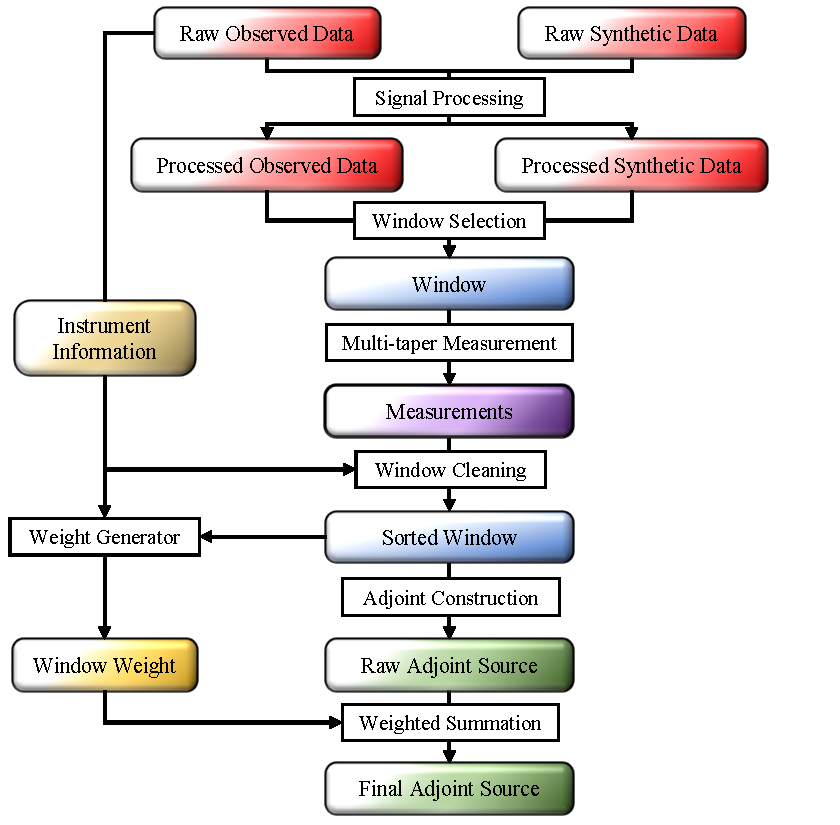
\includegraphics[width=0.8\textwidth]{ch-GLADM25/figures/Preprocess_workflow.pdf}
  \caption[Sub-workflow for pre-processing seismic data]
  {\small{Sub-workflow for pre-processing seismic data.}}
  \label{fig:preprocess_workflow}
\end{figure}

Python provides a great community environment and open-source support,
meaning that for most
of the lower level implementations we do not need write code, but
just find the right Python library.
For example,
Numpy and Scipy support common numerical and matrix operations.
For time series analysis,
Obspy is a Python-based seismic data analysis toolkit which provides
most signal processing operations, such as tapering, demeaning, detrending, filtering, and instrument response removal.
It is far more powerful than SAC,
providing rich APIs, including support for more versatile I/O methods, reading
various source formats (such as NDK, CMTSOLUTION, and QuakeML),
station formats (RESP, pole-zeros, StationXML),
and seismic data formats (e.g., SAC, MSEED, SEGY).
Also, ASDF uses HDF5 as the underlying data container,
and HDF5 already has numerous stable Python libraries, such as h5py,
to read and write HDF5 files in a serial or parallel manner.

Importantly, it is very easy to develop processing tools in a modular style in Python.
Integration of open-source Python packages,
such as Numpy, Scipy, and Obspy, takes much
less effort than writing in Fortran or C, thanks to Python's dynamic language features.
Python also provides and encourages use of very powerful software management systems,
such as pip and Anaconda,
and these tools come with version control capabilities.
All of these attriutes make it much simpler to develop tools in Python than in
Fortran, C, or C++.

There are some disadvantages to using Python.
A common complaint is lack of efficiency due to its dynamic nature.
Python will likely never match the performance of static compiled languages,
such as Fortran or C.
However,
frequently there are other factors that are more critical than speed,
such as fast development, easy deployment, and a user-friendly development environment.
For these reasons, Python has gained much popularity in data science and machine learning, where researchers rely extensively on Python to process big datasets.

In the following, we focus on software we developed
for the data processing workflow, which constitutes the preprocessing phase of the overall adjoint tomography workflow.

\subsection{Software}

\begin{figure}
  \centering
  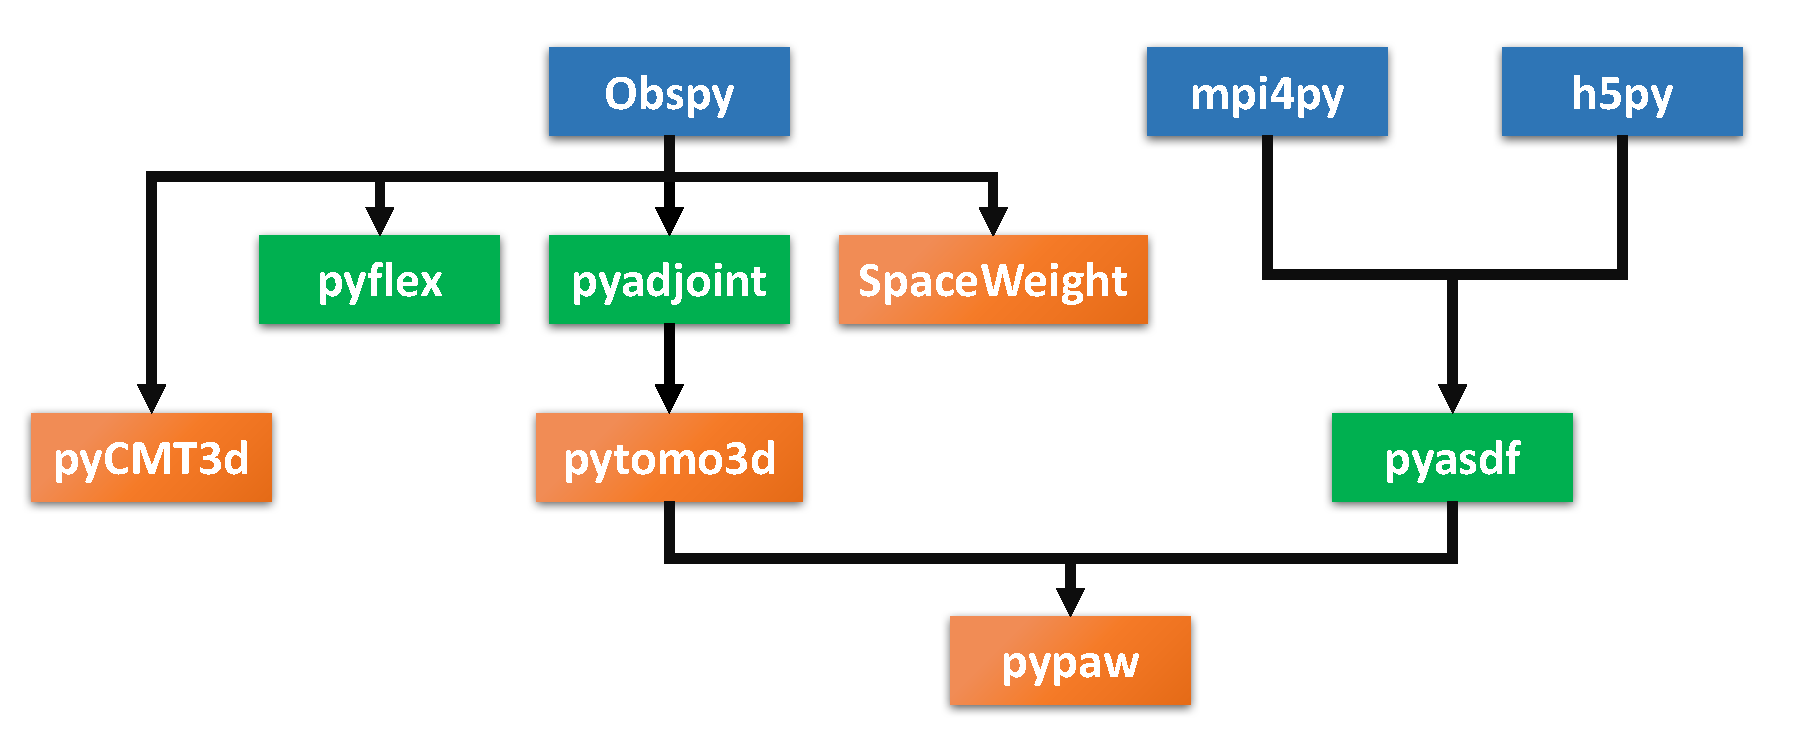
\includegraphics[width=0.98\textwidth]{ch-tools/figures/data_processing_software.pdf}
  \caption[software built for preprocessing seismic data]
  {\small{Software built for preprocessing seismic data. The position and arrows denote software dependencies. Colors denote the contribution level. Software with
  an orange box was mainly developed by me, while Greens boxes signify software I have contributed to, and blue boxes denote common open-source libraries (there are many open-source libraries we use; only major ones are listed.). All the software I developed is open source.}}
  \label{fig:preprocess_software}
\end{figure}


Fig.~\ref{fig:preprocess_software} shows the software tree we developed
for the seismic data processing workflow.
Obspy sits at the lowest level of the processing chain.
It provides APIs for operations on time series data. It is also used for
parsing QuakeML and StationXML files, rotating horizontal seismometer components, calculating arrival times and source and receiver azimuths, etc.
On top of Obspy we developed pycmt3d, pyflex, pyadjoint, and Spaceweight.
Pyflex, the Python version of the Fortran window selection tool FLEXWIN, is used to select time windows on a pair of observed
and synthetic traces.
A new feature we added to Pyflex is seismic
phase detection.
When selecting windows, Pyflex not only identifies seismic phases
based on arrival time calculations, it can also sort windows based on those phases.
This is very convenient when we only wish to select body waves during the window selection stage.
Pyadjoint, the Python port of measure\_adj, is used to make
various types of measurements and construct corresponding adjoint sources.
Spaceweight is a new software package to determine geographical source and stations weights,
which are attached to the adjoint sources and incorporated in the misfit function.
The package is mainly used for
balancing the uneven distribution of sources and stations (see Chapter~\ref{ch:weighting}).
Pycmt3d is a Python port of the Fortran package CMT3D used for seismic source inversions
In addition
to waveform misfits, an option for using envelope misfits has been built into the package,
and geographical weights based on spaceweight can also be assigned as part of the source inversion.

The Python package pytomo3d was created as a higher-level toolkit that integrates
pyflex, pyadjoint, spaceweight, and other utility functions.
Whereas pyflex and pyadjoint operate on the time series provide by obspy as
obspy.trace (one trace is one time series),
pytomo3d operates on a collection of time series provided by obspy as obspy.stream (one stream contains several traces, and in our case one stream
contains traces from the same station).
It is very natural for operations to be
applied at the stream level.
For example, rotating the two horizontal components 
from North and East to radial and transverse is one step in the signal processing
chain.
Basically, the stream options adds another level of abstraction.
Users only need to use APIs provided by pytomo3d,
rather than APIs from lower-level package.
If some lower-level packages become obsolete in the future, for example, pyflex might be
replaced by a more advanced window selection algorithm based on artificial intelligence,
users may not even be aware of that as long as we keep the APIs in pytomo3d unchanged. 
Those who do not use ASDF can utilize all the functionality provided by
pytomo3d and construct their own workflow, since pytom3d has no dependency on ASDF.

For the data container pyasdf branch, mpi4py and h5py sit at the lowest level. mpi4py is the Python version of MPI and handles messaging passing in a parallel environment.
H5py is a Python library for reading and writing hdf5 files.
Based on those libraries (there are more libraries we use, but here we mention the most important ones), we built
pyASDF, which provides the Python APIs for I/O based on ASDF.

At the top level, pypaw combines the data container and processing utility branches
by providing APIs for processing ASDF files during the data processing workflow.
It is used as part of the workflow management tools, which are discussed in the next section.

\section{Workflow Management}
\label{section:workflow_management}

The discussion thus far has focused on improvements of specific parts of the overall tomographic workflow,
such as the data format and time series analysis.
However, the volume of data and the magnitude of the numerical calculations
pose significant challenges for the overall workflow,
because hardware failures become inevitable, and human-induced errors are unavoidable.
The goal of using workflow management tools is to glue the entire inversion process together in a robust and stable fashion.
The main goal of workflow management tools is to use automation to
reduce human interference and errors.
In our global inversion,
we need to manage tens of thousands of ASDF files during each processing stage,
not to mention parameter and configuration files associated with
each data file. It is simply an impossible task to manage and monitor
manually.

By introducing workflow management tools,
we only need to setup the input and output
patterns for each processing stage, and data should
follow these patterns regardless of volume.
This has the additional benefit of reducing the overall time to solution for each iteration, since
each component can be connected without time gaps. 

Another benefit of workflow management is an increase in the robustness of the system.
With thousands of earthquakes and millions of seismic traces,
our inversion severely stresses compute nodes and the file system, and there are occasional hardware failures which cause jobs to fail.
Workflow management tools should have the capability to
detect such failures and recover from them.
Only jobs which pass validation may be labeled as completed and continue to the next stage of processing.

After exploring several existing workflow management tools,
we selected the Ensemble ToolKit (EnTK)~\cite{EnTK2017} developed by the RADICAL
group from Rutgers University.
In this environment,
the simpy (Seismic Inversion Management PYthon) toolkit was developed using RADICAL-SAGA, pypaw, and sqlite3.
RADICAL-SAGA works as the 
job management component responsible for communicating with the queue of the HPC system,
pypaw provides user-defined processing components,
and sqlite3 is used as a bookkeeping database to keep track of job statuses.

Before the start of processing,
simpy validates all input and parameter files and stores them
into the sqlite3 database.
All initial jobs are labeled as `new'.
As the workflow starts, simpy submits jobs using 
RADICAL-SAGA as the job manager engine to communicate with the HPC system.
As soon as a job finishes, simpy receives notifications from
RADICAL-SAGA and launches a job validation process.
Once job passes validation,
it labels the job as `done' in the database.
If the job fails, simpy labels
the job status according to the error type and re-submit failed jobs in batch mode.
By utilizing existing tools like RADICAL-SAGA, we only need to focus on the user logic rather
than job management, thereby offloading work to those libraries.
RADICAL-SAGA has the capability to communicate with many job submission systems,
so it can potentially be deployed on many other supercomputer systems without any
code changes (although some configuration changes may still be required).

As a most recent development, we integrated EnTK
into our forward and adjoint simulation workflows. Our ultimate
goad is to develop a workflow tool that works across platforms and integrates one entire tomographic iteration, including forward simulations, data processing, adjoin simulations, and post-processing.
